\documentclass[10pt]{article}
\usepackage[utf8]{inputenc}
\usepackage{mathptmx}
\usepackage{tabularx}
\usepackage{fancyvrb}
\usepackage{graphicx}
\usepackage{amsmath}
\usepackage{siunitx}
\usepackage{subcaption}
\usepackage[top=19mm, bottom=43mm, left=12.925mm, right=12.925mm, a4paper]{geometry}
\usepackage{hyperref}
\usepackage{xcolor}
\hypersetup{
    pdfpagelabels=true,
    plainpages=false,
    pdfauthor={Søren Bøgeskov Nørgaard, Henrik Aarup Vesterager, Lasse Thomsen},
    pdftitle={AAU Plot Library},
    pdfsubject={},
    bookmarksdepth=3,
    bookmarksnumbered=true,
    colorlinks,
    citecolor=black,
    filecolor=black,
    linkcolor=black,
    urlcolor=black,
    pdfstartview=FitH
}

\title{AAU Plot Library}
\author{Søren B.\ Nørgaard, Henrik A.\ Vesterager, Lasse Thomsen}
\begin{document}
\maketitle

\begin{abstract}
    The functions of this module makes it easy to plot consistent figures for the report.
\end{abstract}

\tableofcontents


\section{Files}
\begin{tabularx}{\linewidth}{lX}
    \texttt{aauplot.py} & Library file. \\
\end{tabularx}

\section{Installation}
\begin{enumerate}
\item Make sure to install Python 3, numpy, scipy, and matplotlib.
\item Put the library files in a central directory (e.g.\ \texttt{C:/PathTo/Something}).
\item Add this path to the environment variable \texttt{PYTHONPATH} (\emph{Environment Variables} in Windows and \texttt{.bashrc} or \texttt{.profile} in Linux/OSX). E.g.\
    \begin{verbatim}
# ~/.profile
export PYTHONPATH=$PYTHONPATH:/home/soren/hdd/svn/project9-10/scripts/lib
    \end{verbatim}
\end{enumerate}


\section{Modules}
\subsection{Satimo}
\subsubsection{col2mat(column, ntheta=SATIMO\_NUM\_ELEVATION, nphi=SATIMO\_NUM\_AZIMUTH)}
Convert a Satimo PM-exported column to a matrix with phi the 
x-axis and theta on the y-axis.

\begin{verbatim}
- column: Column from a Satimo PM export.
- ntheta: Number of rows in the output (theta in the input).
- nphi: Number of columns in the output (phi in the input).

Return:
Matrix with phi on the x-axis and theta on the y-axis.
\end{verbatim}

\subsubsection{efficiency(trxfile, calfiles, reffiles)}
Get the total efficiency of a trx file, exported from Satimo.

\begin{verbatim}
- trxfile: File, exported from Satimo PM, to compute the efficiency of.
- calfiles: List of calibration measurement files (trx files).
- reffiles: List of reference files relating to the calibration
        measurements.

Return:
[f,eff] -- the total efficiency, eff, for each frequency, f.
\end{verbatim}

\subsubsection{loadref(f)}
Load a reference file containing S11, Gain, and Efficiency of a
reference/calibration antenna.

\begin{verbatim}
- f: File name.

Return:
M[0]=frequency(Hz), M[1]=S11(.), M[2]=Gain(.), M[3]=Eff(.)
\end{verbatim}

\subsubsection{loadtrx(f)}
Load a trx measurement file from Satimo PM into memory. 

\begin{verbatim}
- f: TRX file to load.

Return:
[f, list_horiz, list_vert] where
        f = [f1, f2, f3, ...]
        list_horiz = [E_horiz_f1, E_horiz_f2, E_horiz_f3, ...]
        list_vert  = [E_vert_f1,  E_vert_f2,  E_vert_f3,  ...]
and each "E" is a complex matrix, (theta x phi), containing the received fields.
\end{verbatim}

\subsubsection{radiatedpower(h,v)}
Compute the radiated power for each frequency in the h and v list, using
radiatedpower\_single().

\begin{verbatim}
- h: List of complex (theta x phi) matrices -- one for each frequency.
        Horizontal polarization.
- v: List of complex (theta x phi) matrices -- one for each frequency.
        Vertical polarization.

Return:
A vector with the radiated power for each frequency/element of h and
        v.
\end{verbatim}

\subsubsection{radiatedpower\_single(Etot)}
Radiated power from a (theta x phi) total E-field matrix.

\begin{verbatim}
- Etot: Matrix (theta x phi) from Satimo PM to compute the radiate power
        of (surface integration).

Return:
Surface integral of Etot ~ radiated power.
\end{verbatim}

\subsubsection{totalpower\_table(calfiles, reffiles)}
Make a table of calibrated "total power" for each frequency.
Having (1) the total power and (2) the radiated power for a given antenna,
makes it possible to compute the total efficiency of the antenna.

\begin{verbatim}
- calfiles: List of calibration measurement files (trx files) (order:
        lowest to highest frequency).
- reffiles: List of reference files relating to the calibration
        measurements (order: lowest to highest frequency).

Return:
[f,Ptot] -- the total power for each frequency.
\end{verbatim}

\clearpage
\subsection{CST}
\subsubsection{col2mat(column, nx=360, ny=181)}
Convert a CST-exported column to a matrix with phi the 
x-axis and theta on the y-axis.

\begin{verbatim}
- column: Column from a Satimo export.
- nx: Number of columns in the output (phi in the input).
- ny: Number of rows in the output (theta in the input).

Return:
Matrix with phi on the x-axis and theta on the y-axis.
\end{verbatim}

\subsubsection{loadff(f)}
Load a CST exported file to two (theta x phi) matrices -- one for theta and
one for phi plarization.

\begin{verbatim}
- f: File to load.

Return:
[T,P] where T and P are each a (theta x phi) matrix.
\end{verbatim}

\clearpage
\subsection{L3D}
\subsubsection{ecc(Eth1, Eth2, Eph1, Eph2)}
Compute the envelope correlation coefficient between two farfields. The
farfields are split into theta and phi part. Each part is a matrix with
theta on one axis and phi on the other.

\begin{verbatim}
- Eth1: E-field, theta part, antenna 1
- Eth2: E-field, theta part, antenna 2
- Eph1: E-field, phi part, antenna 1
- Eph1: E-field, phi part, antenna 2

Return:
Envelope Correlation Coefficient (scalar)

Note:
https://mns.ifn.et.tu-dresden.de/Lists/nPublications/Attachments/612/Wang_Q_WSA_10.pdf
\end{verbatim}

\subsubsection{intsphere(r, theta, phi)}
Do a spherical integral of a theta-phi matrix.

\begin{verbatim}
- r: Matrix to integrate (x-axis=phi, y-axis=theta).
- phi: Phi axis values.
- theta: Theta axis values.

Return:
Scalar result of the integration.
\end{verbatim}

\subsubsection{plot3d(r, stride=1, th\_lim=(0, pi), ph\_lim=(0, 2*pi))}
Plot a matrix, (theta x phi), in 3d space.

\begin{verbatim}
- r: Matrix to plot.
- stride: Resolution of the output. 1=detailed+slow, 10=rough+fast.
- th_lim: Upper and lower theta limits.
- ph_lim: Upper and lower phi limits.
\end{verbatim}

\subsubsection{plotflat(r, th\_lim=(0,pi), ph\_lim=(0,2*pi), cmap="jet")}
Plot a farfield-matrix as a color-map. Remember that 0 degrees is the bottom
of the plot in spherical coordinates.

\begin{verbatim}
- r: Matrix to plot (theta x phi).
- th_lim: Minimum and maximum theta/y-axis value.
- ph_lim: Minimum and maximum phi/x-axis value.
- cmap: Color map to use.
\end{verbatim}



\clearpage
\section{Examples}

\subsection{Plot S-Parameters}

S-parameters can be easily plotted using a script like the one below. The result is shown in Figure~\ref{fig:example1}.
\VerbatimInput{examples/ex1.py}

\begin{figure}[htbp]
    \centering
    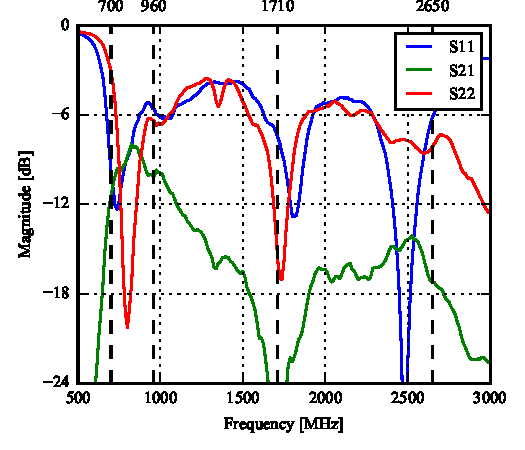
\includegraphics{examples/ex1_sparams.pdf}
    \caption{S-parameters.}
    \label{fig:example1}
\end{figure}

\end{document}
